%%%%%%%%%%%%%%%%%%%%%%%%%%%%%%%%%%%%%%%%%%%%%%%%%%%%%%%%%%%%%%%%%%%%%
%% This is a (brief) model paper using the achemso class
%% The document class accepts keyval options, which should include
%% the target journal and optionally the manuscript type.
%%%%%%%%%%%%%%%%%%%%%%%%%%%%%%%%%%%%%%%%%%%%%%%%%%%%%%%%%%%%%%%%%%%%%
\documentclass[journal=jpcbfk,manuscript=article]{achemso}

%\documentclass[english,aps,preprint,pre,floatfix,nofootinbib,showpacs,showkeys]{revtex4-1}
%%%%%%%%%%%%%%%%%%%%%%%%%%%%%%%%%%%%%%%%%%%%%%%%%%%%%%%%%%%%%%%%%%%%%
%% Place any additional packages needed here.  Only include packages
%% which are essential, to avoid problems later. Do NOT use any
%% packages which require e-TeX (for example etoolbox): the e-TeX
%% extensions are not currently available on the ACS conversion
%% servers.
%%%%%%%%%%%%%%%%%%%%%%%%%%%%%%%%%%%%%%%%%%%%%%%%%%%%%%%%%%%%%%%%%%%%%
\usepackage[version=3]{mhchem} % Formula subscripts using \ce{}

\SectionNumbersOn

\usepackage{amsmath}
\usepackage{amssymb}
\usepackage{color}
\usepackage{CJK}https://www.overleaf.com/project/5e820b28d741e00001b1ccac
\usepackage{framed}
\usepackage[hidelinks]{hyperref}
\usepackage{algorithm}
\usepackage{algpseudocode}
\algdef{SE}[DOWHILE]{Do}{doWhile}{\algorithmicdo}[1]{\algorithmicwhile\ #1}

\usepackage[scaled=0.85]{beramono}
\usepackage[T1]{fontenc}
\usepackage{changepage}

%%%%%%%%%%%%%%%%%%%%%%%%%%%%%%%%%%%%%%%%%%%%%%%%%%%%%%%%%%%%%%%%%%%%%
%% If issues arise when submitting your manuscript, you may want to
%% un-comment the next line.  This provides information on the
%% version of every file you have used.
%%%%%%%%%%%%%%%%%%%%%%%%%%%%%%%%%%%%%%%%%%%%%%%%%%%%%%%%%%%%%%%%%%%%%
%%\listfiles

%%%%%%%%%%%%%%%%%%%%%%%%%%%%%%%%%%%%%%%%%%%%%%%%%%%%%%%%%%%%%%%%%%%%%
%% Place any additional macros here.  Please use \newcommand* where
%% possible, and avoid layout-changing macros (which are not used
%% when typesetting).
%%%%%%%%%%%%%%%%%%%%%%%%%%%%%%%%%%%%%%%%%%%%%%%%%%%%%%%%%%%%%%%%%%%%%

\makeatletter
    \setlength\@fptop{0\p@}
\makeatother

\newcommand*\mycommand[1]{\texttt{\emph{#1}}}

\newcommand{\state}[1]{$\mathcal{S}_{#1}$}

%\newcommand*{\rood}[1]{\textcolor{red}{#1}}
\newcommand*{\rood}[1]{#1}
%\newcommand*{\blauw}[1]{\textcolor{blue}{#1}}
\newcommand*{\blauw}[1]{#1}
%\newcommand*{\groen}[1]{\textcolor{green}{#1}}
\newcommand*{\groen}[1]{#1}
%\newcommand*{\blauwr}[1]{\textcolor{blue}{#1}}
\newcommand*{\blauwr}[1]{#1}

%\newcommand*{\addref}[1]{\textcolor{red}{\{ADD REF: #1\}}}

%\newcommand*{\noter}[1]{\textcolor{red}{[[#1]]}}		% notes on
\newcommand*{\noter}[1]{}					% notes off

%\usepackage[draft]{todonotes}   % notes shown
\usepackage[disable]{todonotes} % notes hidden

%%%%%%%%%%%%%%%%%%%%%%%%%%%%%%%%%%%%%%%%%%%%%%%%%%%%%%%%%%%%%%%%%%%%%
%% Meta-data block
%% ---------------
%% Each author should be given as a separate \author command.
%%
%% Corresponding authors should have an e-mail given after the author
%% name as an \email command. Phone and fax numbers can be given
%% using \phone and \fax, respectively; this information is optional.
%%
%% The affiliation of authors is given after the authors; each
%% \affiliation command applies to all preceding authors not already
%% assigned an affiliation.
%%
%% The affiliation takes an option argument for the short name.  This
%% will typically be something like "University of Somewhere".
%%
%% The \altaffiliation macro should be used for new address, etc.
%% On the other hand, \alsoaffiliation is used on a per author basis
%% when authors are associated with multiple institutions.
%%%%%%%%%%%%%%%%%%%%%%%%%%%%%%%%%%%%%%%%%%%%%%%%%%%%%%%%%%%%%%%%%%%%%
\author{Mike Jones}
\affiliation{%
  Pritzker School of Molecular Engineering, %
  University of Chicago, %
  Chicago, Illinois 60637%
}

\author{Andrew L. Ferguson}
\email{andrewferguson@uchicago.edu}
\affiliation{%
  Pritzker School of Molecular Engineering, %
  University of Chicago, %
  Chicago, Illinois 60637%
}
%\author{I. Ken Groupleader}
%\altaffiliation{A shared footnote}
%\email{i.k.groupleader@unknown.uu}
%\phone{+123 (0)123 4445556}
%\fax{+123 (0)123 4445557}
%\affiliation[Unknown University]
%{Department of Chemistry, Unknown University, Unknown Town}
%\alsoaffiliation[Second University]
%{Department of Chemistry, Second University, Nearby Town}

%\author{Susanne K. Laborator}
%\email{s.k.laborator@bigpharma.co}
%\affiliation[BigPharma]
%{Lead Discovery, BigPharma, Big Town, USA}

%\author{Kay T. Finally}
%\affiliation[Unknown University]
%{Department of Chemistry, Unknown University, Unknown Town}
%\alsoaffiliation[Second University]
%{Department of Chemistry, Second University, Nearby Town}

%%%%%%%%%%%%%%%%%%%%%%%%%%%%%%%%%%%%%%%%%%%%%%%%%%%%%%%%%%%%%%%%%%%%%
%% The document title should be given as usual. Some journals require
%% a running title from the author: this should be supplied as an
%% optional argument to \title.
%%%%%%%%%%%%%%%%%%%%%%%%%%%%%%%%%%%%%%%%%%%%%%%%%%%%%%%%%%%%%%%%%%%%%
\title[]{TBA}


%%%%%%%%%%%%%%%%%%%%%%%%%%%%%%%%%%%%%%%%%%%%%%%%%%%%%%%%%%%%%%%%%%%%%
%% Some journals require a list of abbreviations or keywords to be
%% supplied. These should be set up here, and will be printed after
%% the title and author information, if needed.
%%%%%%%%%%%%%%%%%%%%%%%%%%%%%%%%%%%%%%%%%%%%%%%%%%%%%%%%%%%%%%%%%%%%%
%\abbreviations{IR -- infrared, NMR -- nuclear magnetic resonance, UV -- ultraviolet}
%\keywords{Takens}

\begin{document}
%%%%%%%%%%%%%%%%%%%%%%%%%%%%%%%%%%%%%%%%%%%%%%%%%%%%%%%%%%%%%%%%%%%%%
%% The manuscript does not need to include \maketitle, which is
%% executed automatically.  The document should begin with an
%% abstract, if appropriate.  If one is given and should not be, the
%% contents will be gobbled.
%%%%%%%%%%%%%%%%%%%%%%%%%%%%%%%%%%%%%%%%%%%%%%%%%%%%%%%%%%%%%%%%%%%%%

\newpage

\begin{abstract}

\noindent 

\end{abstract}
https://www.overleaf.com/project/5e9e5110c524b8000192c548
%%%%%%%%%%%%%%%%%%%%%%%%%%%%%%%%%%%%%%%%%%%%%%%%%%%%%%%%%%%%%%%%%%%%%
%% Start the main part of the manuscript here.
%%%%%%%%%%%%%%%%%%%%%%%%%%%%%%%%%%%%%%%%%%%%%%%%%%%%%%%%%%%%%%%%%%%%%

\newpage

\section{\label{sec:intro}Introduction}

DNA motivation
\begin{enumerate}
	\item Connection to Tokmakoff results
	\item Some origami, sensor, other nanotech appications
\end{enumerate}
	
SRV motivation
\begin{enumerate}
	\item First time studying a two body problem
	\item Compare with other TICA-MSM approaches to DNA
	\item Compare with Noe nucleotide paper
\end{enumerate}

\section{\label{sec:methods}Methods}

Simulation set up

Featurization
\begin{enumerate}
	\item Vamp-2 score for permutable distances is slightly lower but should not contain degenerate information (SI data)
	\item Inverse distances have higher vamp-2 score than regular distances (SI data)
\end{enumerate}

SRV validation
\begin{enumerate}
	\item Plot loss scores and self-consistency check for each sequence (fig 1 and 2)
	\item Select number of slow modes (different for each) and lag time (same for each) based on this analysis.
	\item Only use off diagonals and add sequence visuals along axes (fig 3)
\end{enumerate}

MSM construction
\begin{enumerate}
	\item hyperparameters include: number of microstates, lag (use same as SRV), number of macrostates (usually n+1) but we use n states for GC-core and GC-mid. I have not done a full optimization sweep over these parameters, but can explain the motivation for choosing these.
    \item Can show comparison data with TICA -- timescales converge faster and state assignments tend to be more concrete (although this has varied) (fig 4)
\end{enumerate}  

\section{\label{sec:methods}Discussion}

Brief description and diagrams for collective variables:
\begin{enumerate}
	\item Inverse average shifting distance
	\item Fourth basepair distances
\end{enumerate} 

AT-all
\begin{enumerate}
	\item Dynamics dominated by slow shifting modes
	\item sources to verify this would be the case
	\item Minimal data from Tokmakoff on this, but can look at relative hybridization rates
	\item SI Calculations to prove preferred thermo stability of 5’ shifted state
\end{enumerate}  

GC-end
\begin{enumerate}
	\item Similar dynamics to AT-all, but with overall lower stability and timescales
	\item Difficult to make any claims because the thermodynamics of external mismatches with dangling ends have not been measured experimentally, and 3spn2 does not paramertize these mismatches explicitly
	\item According to SantaLucia external mismatches and dangling ends tend to have weakly stabilizing effect, and there are 4-6 intact basepairs for these conformations
	\item Might account for unknown signal in 2018 Tokmakoff paper with timescale between the fraying and dehybrization signal, but not sure... 
\end{enumerate}  

GC-core
\begin{enumerate}
	\item Frayed states requires the fourth base pair to be broken, most partially frayed states are not included in metastable clustering
	\item 2nd slow mode correlates well with expected fraying behavior, can sample along this mode and generally find increasing frayed states (although the SRV coords are spiky)
	\item 3rd mode is reflective of changes in orientation in dissociated behavior. This could be interesting for the SI, but this state does not inform the macrostate clustering
\end{enumerate}  
GC-mid
\begin{enumerate}
	\item Evidence of fraying correlations in higher order modes, but these are not consistent and their inclusion does not generate a metastable third mode
	\item Treat this as a two-states model, where fraying is an expected feature of the hybridized state but not does not characterize a metastable state
\end{enumerate}  
    
\begin{figure}[ht!]
	\begin{center}
        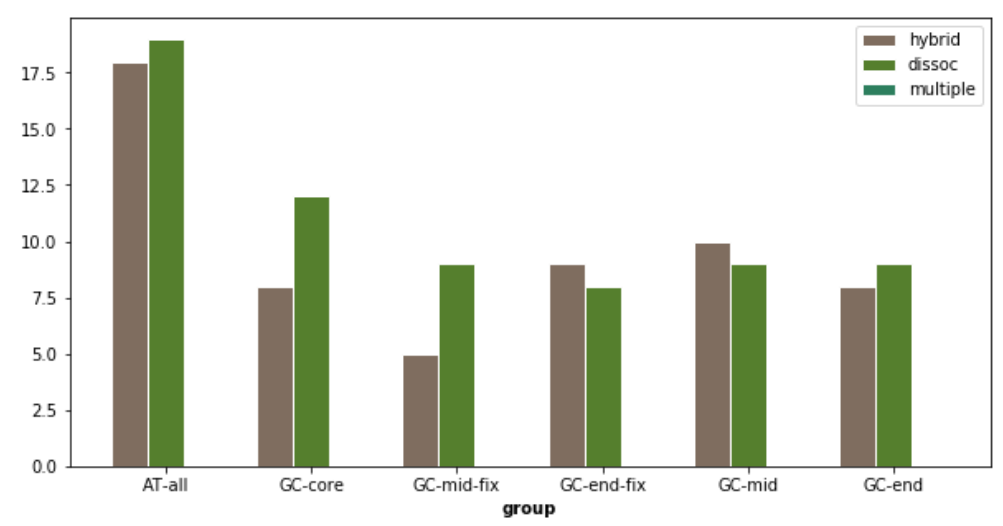
\includegraphics[width=\textwidth]{Figs/skeleton/n_events.PNG}
        \caption{Number of events per sequence. I would only included the four sequences in the actual pub. (this could be supplemental}
        \label{fig:n_events}
	\end{center}
\end{figure}   
    
\begin{figure}[ht!]
	\begin{center}
        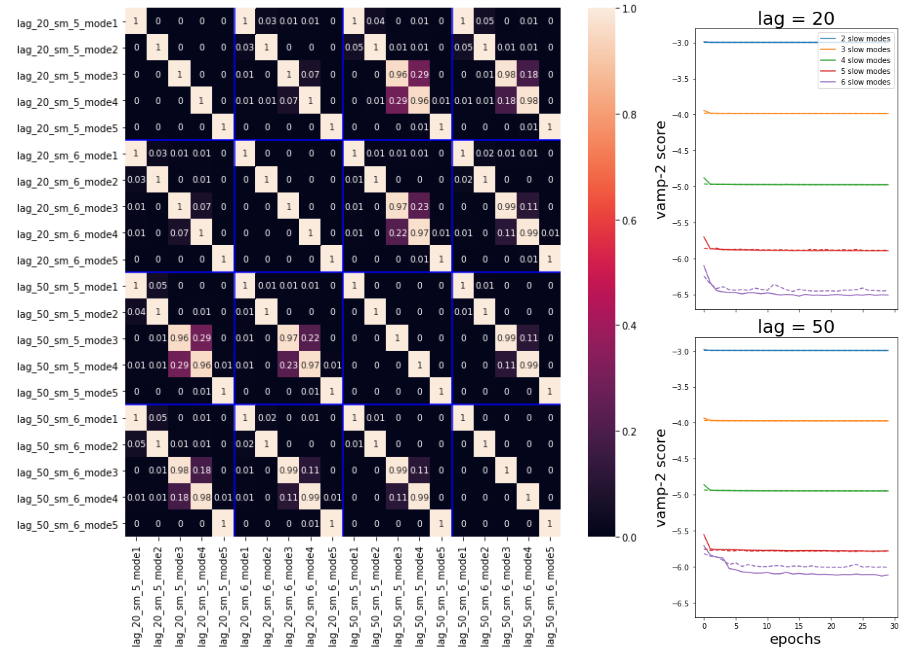
\includegraphics[width=\textwidth]{Figs/skeleton/AT-all_validation.PNG}
        \caption{For Supplemental info: Selection process for AT-all slow modes}
        \label{fig:AT-all_val}
	\end{center}
\end{figure}

\begin{figure}[ht!]
	\begin{center}
        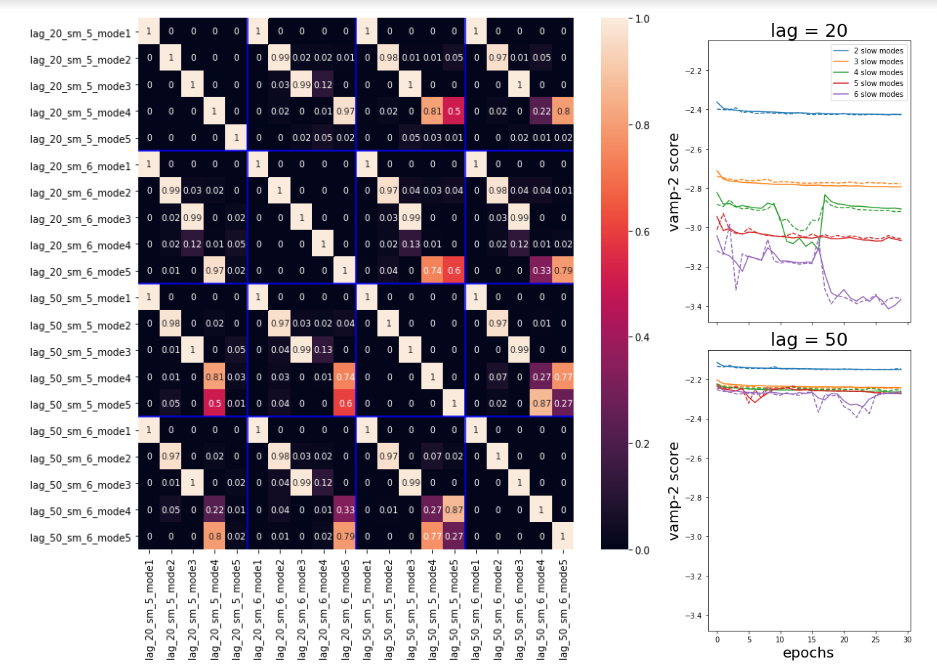
\includegraphics[width=\textwidth]{Figs/skeleton/GC-core_validation.PNG}
        \caption{For Supplemental info: Selection process for GC-core slow modes}
        \label{fig:GC-core_val}
	\end{center}
\end{figure}

\begin{figure}[ht!]
	\begin{center}
        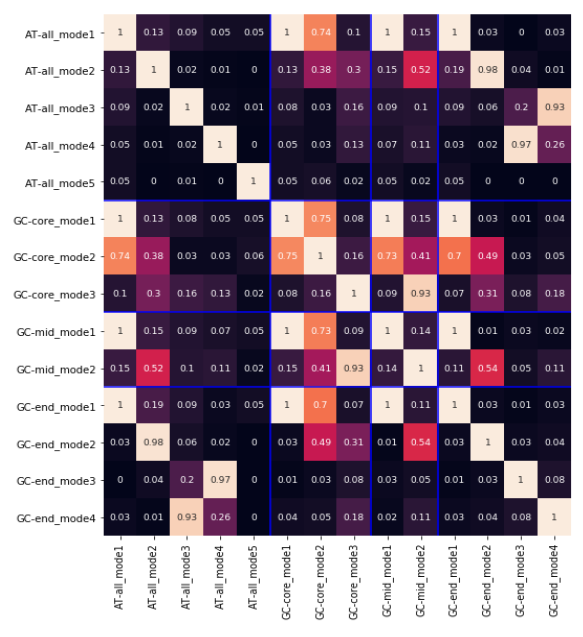
\includegraphics[width=\textwidth]{Figs/skeleton/all_modes_correlations.PNG}
        \caption{For Supplemental info: Correlations between all leading modes}
        \label{fig:all_modes}
	\end{center}
\end{figure}

\begin{figure}[ht!]
	\begin{center}
        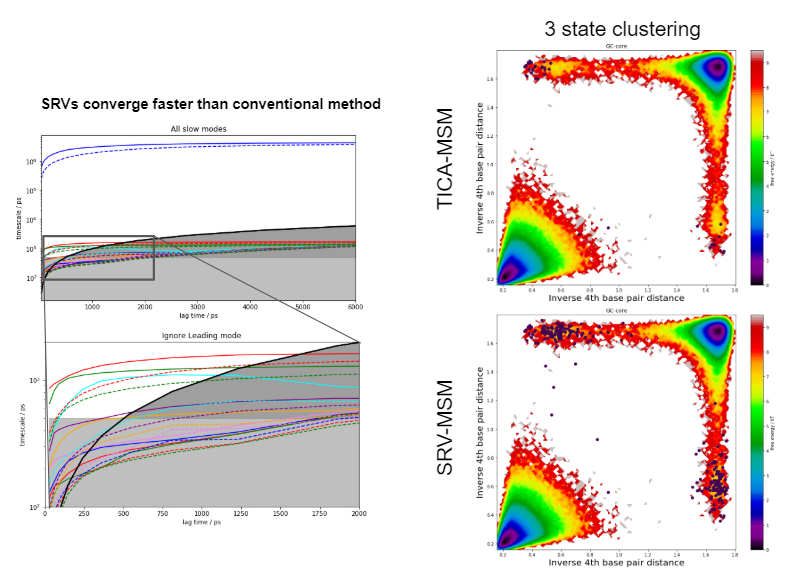
\includegraphics[width=\textwidth]{Figs/skeleton/tica_comparison_GC-core.PNG}
        \caption{SRV vs. TICA MSMs and resulting clsuter memberships}
        \label{fig:tica_comparison}
	\end{center}
\end{figure}

\begin{figure}[ht!]
	\begin{center}
        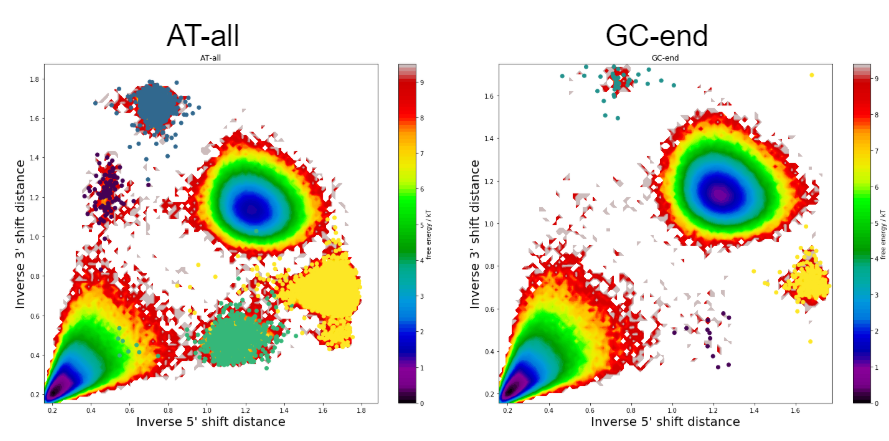
\includegraphics[width=\textwidth]{Figs/skeleton/shifting_distribution.PNG}
        \caption{Shows similarities between shifting modes and state memberships for AT-all and GC-ends}
        \label{fig:shifting_distributions}
	\end{center}
\end{figure}

\begin{figure}[ht!]
	\begin{center}
        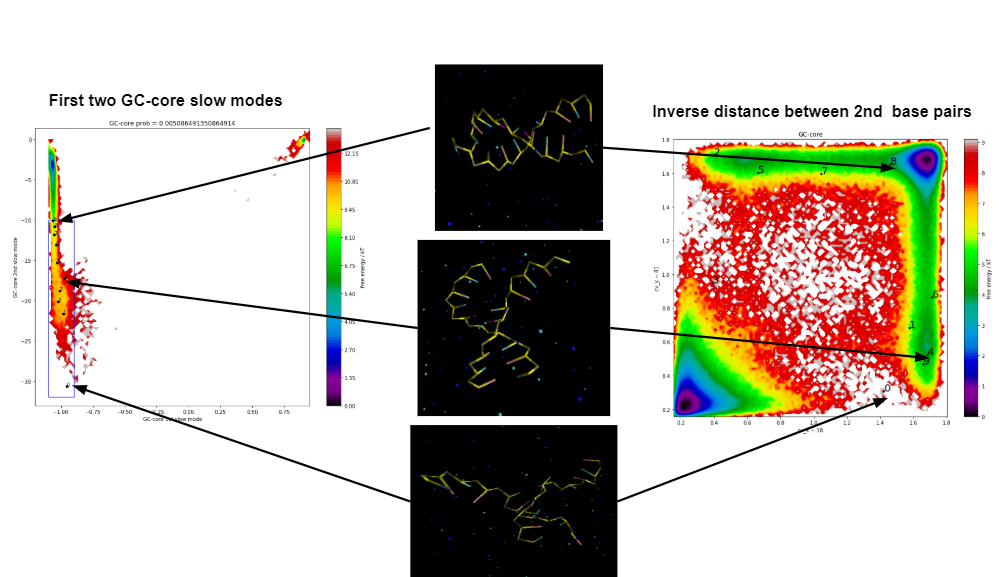
\includegraphics[width=\textwidth]{Figs/skeleton/sample_fray.PNG}
        \caption{Sample along 2nd GC-core SRV mode and show that these have increasing amounts of fraying}
        \label{fig:sample_fray}
	\end{center}
\end{figure}

\begin{figure}[ht!]
	\begin{center}
        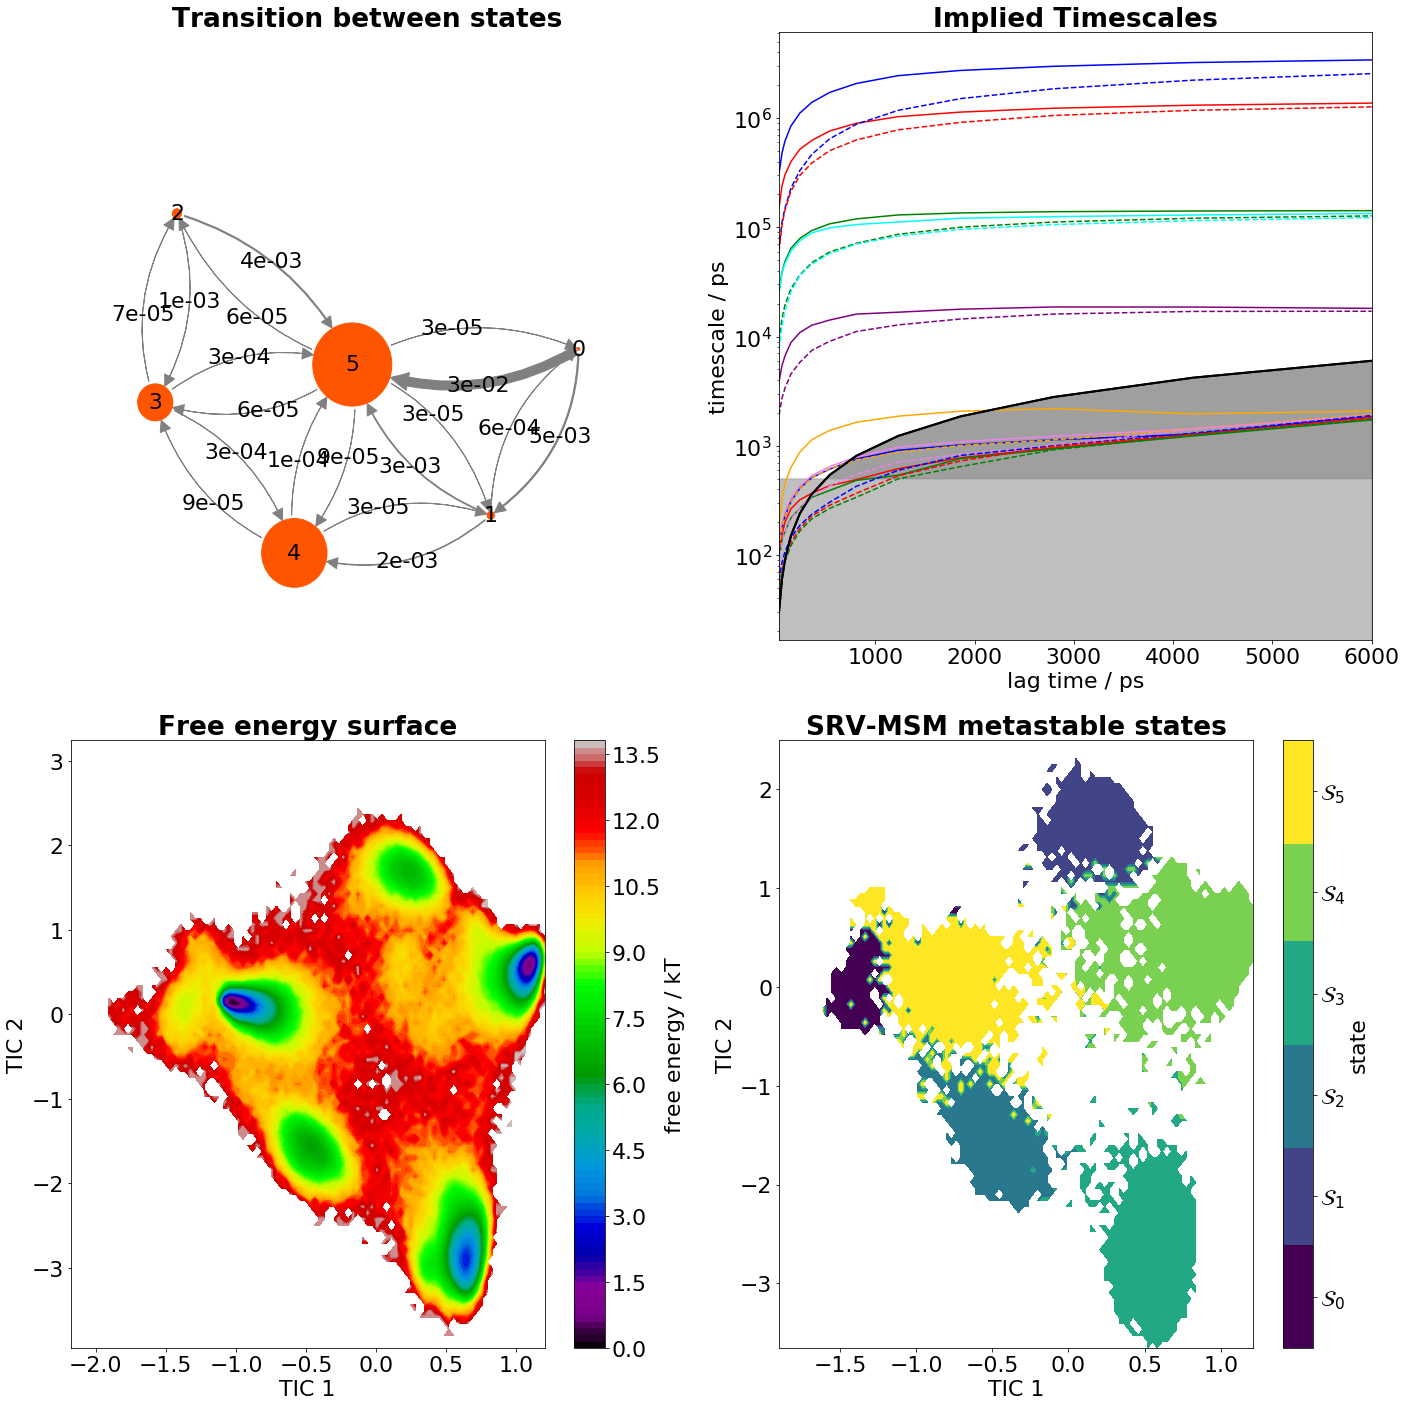
\includegraphics[width=\textwidth]{Figs/skeleton/AT-all_vis.png}
        \caption{AT-all transition diagram, implied timescales between SRV-MSM and TICA-MSM, free energy surface and metastable state assignment.}
        \label{fig:sample_fray}
	\end{center}
\end{figure}

\begin{figure}[ht!]
	\begin{center}
        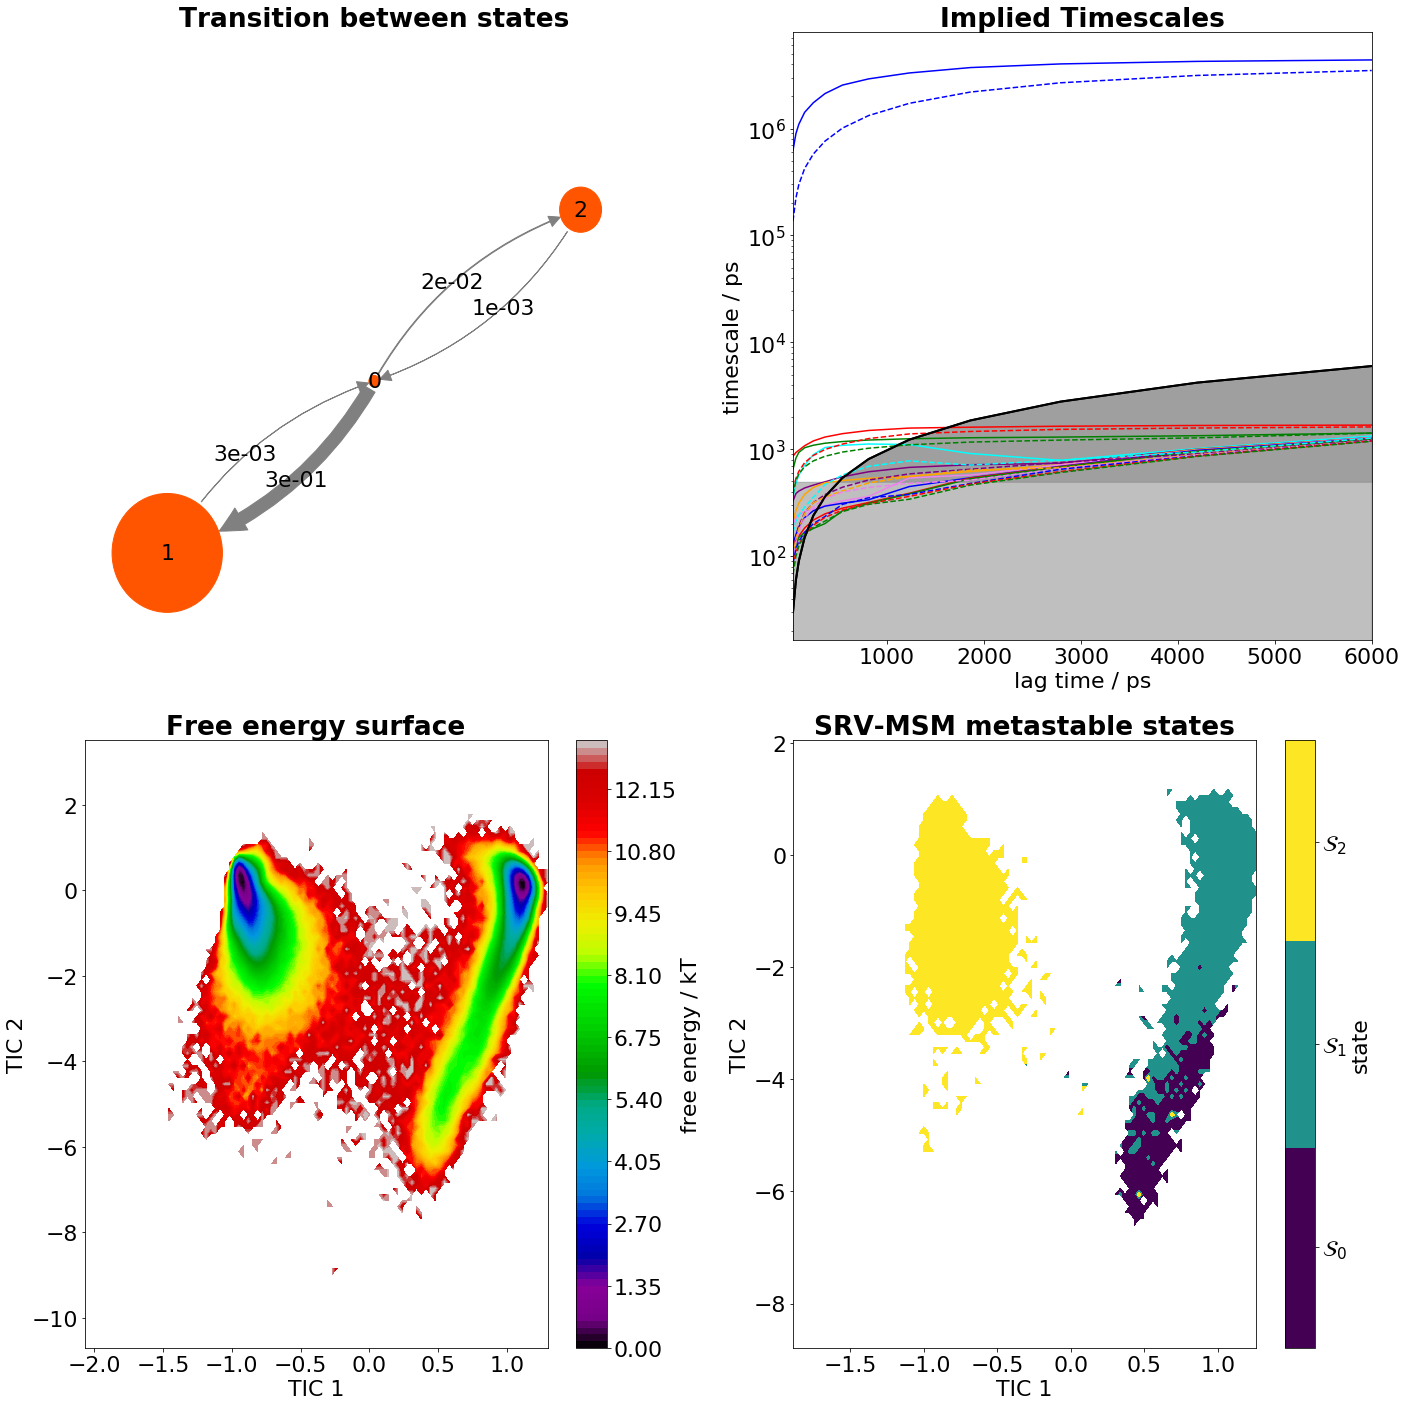
\includegraphics[width=\textwidth]{Figs/skeleton/GC-core_vis.png}
        \caption{GC-core transition diagram, implied timescales between SRV-MSM and TICA-MSM, free energy surface and metastable state assignment.}
        \label{fig:sample_fray}
	\end{center}
\end{figure}

\clearpage
\newpage

\bibliography{references}

%%%%%%%%%%%%%%%%%%%%%%%%%%%%%%%%%%%%%%%%%%%%%%%%%%%%%%%%%%%%%%%%%%%%%
%% The "tocentry" environment can be used to create an entry for the
%% graphical table of contents.
%%%%%%%%%%%%%%%%%%%%%%%%%%%%%%%%%%%%%%%%%%%%%%%%%%%%%%%%%%%%%%%%%%%%%

\clearpage


\end{document}
